\subsubsection{Compara\c c\~ao dos Modelos}

Com o objetivo de obter uma análise mais aprofundada do desempenho de cada modelo, foi realizada uma comparação por meio de um gráfico de violino e de barra. Dessa forma, pôde-se observar qual dos modelos apresentava o melhor desempenho.



Ao examinar os modelos representados nas Figuras \ref{fig:modelos-arima} e \ref{fig:violin-lr-xgb-lgbm-rf}, identifico os modelos que se destacam em relação à natureza dos dados. Na Figura \ref{fig:basic_comparar}, que compara os modelos ARIMA e XGBoost com outros, torna-se evidente que os modelos ARIMA como AR, ARX, MA, ARMA, ARIMAX e SARIMAX demonstram um desempenho sólido. Além disso, os modelos baseados em gradientes e regressão, como o XGBoost, exibem resultados comparáveis, beneficiando-se da otimização por meio do Optuna, uma abordagem de bayesiana usando o metodo TPE.

Na Figura \ref{fig:rrmse_comparar}, que contrasta as redes neurais com o modelo Prophet, é importante destacar que os modelos de redes neurais, incluindo RNN, LSTM, GRU, ANN, CNN e Transformer, foram avaliados em conjunto com o modelo Prophet. A análise estatística também demonstrou que o modelo RNN se sobressai como o vencedor entre as métricas avaliadas. Essa conclusão é respaldada pelas evidências de que pelo menos um modelo é superior aos demais. Os modelos com valores de p-valor abaixo de $0,05$ foram realçados em \textit{itálico} para enfatizar sua significância.

\begin{figure}[!htb]
	\centering
	\caption{Comparação dos modelos ARIMA}\label{fig:modelos-arima}
	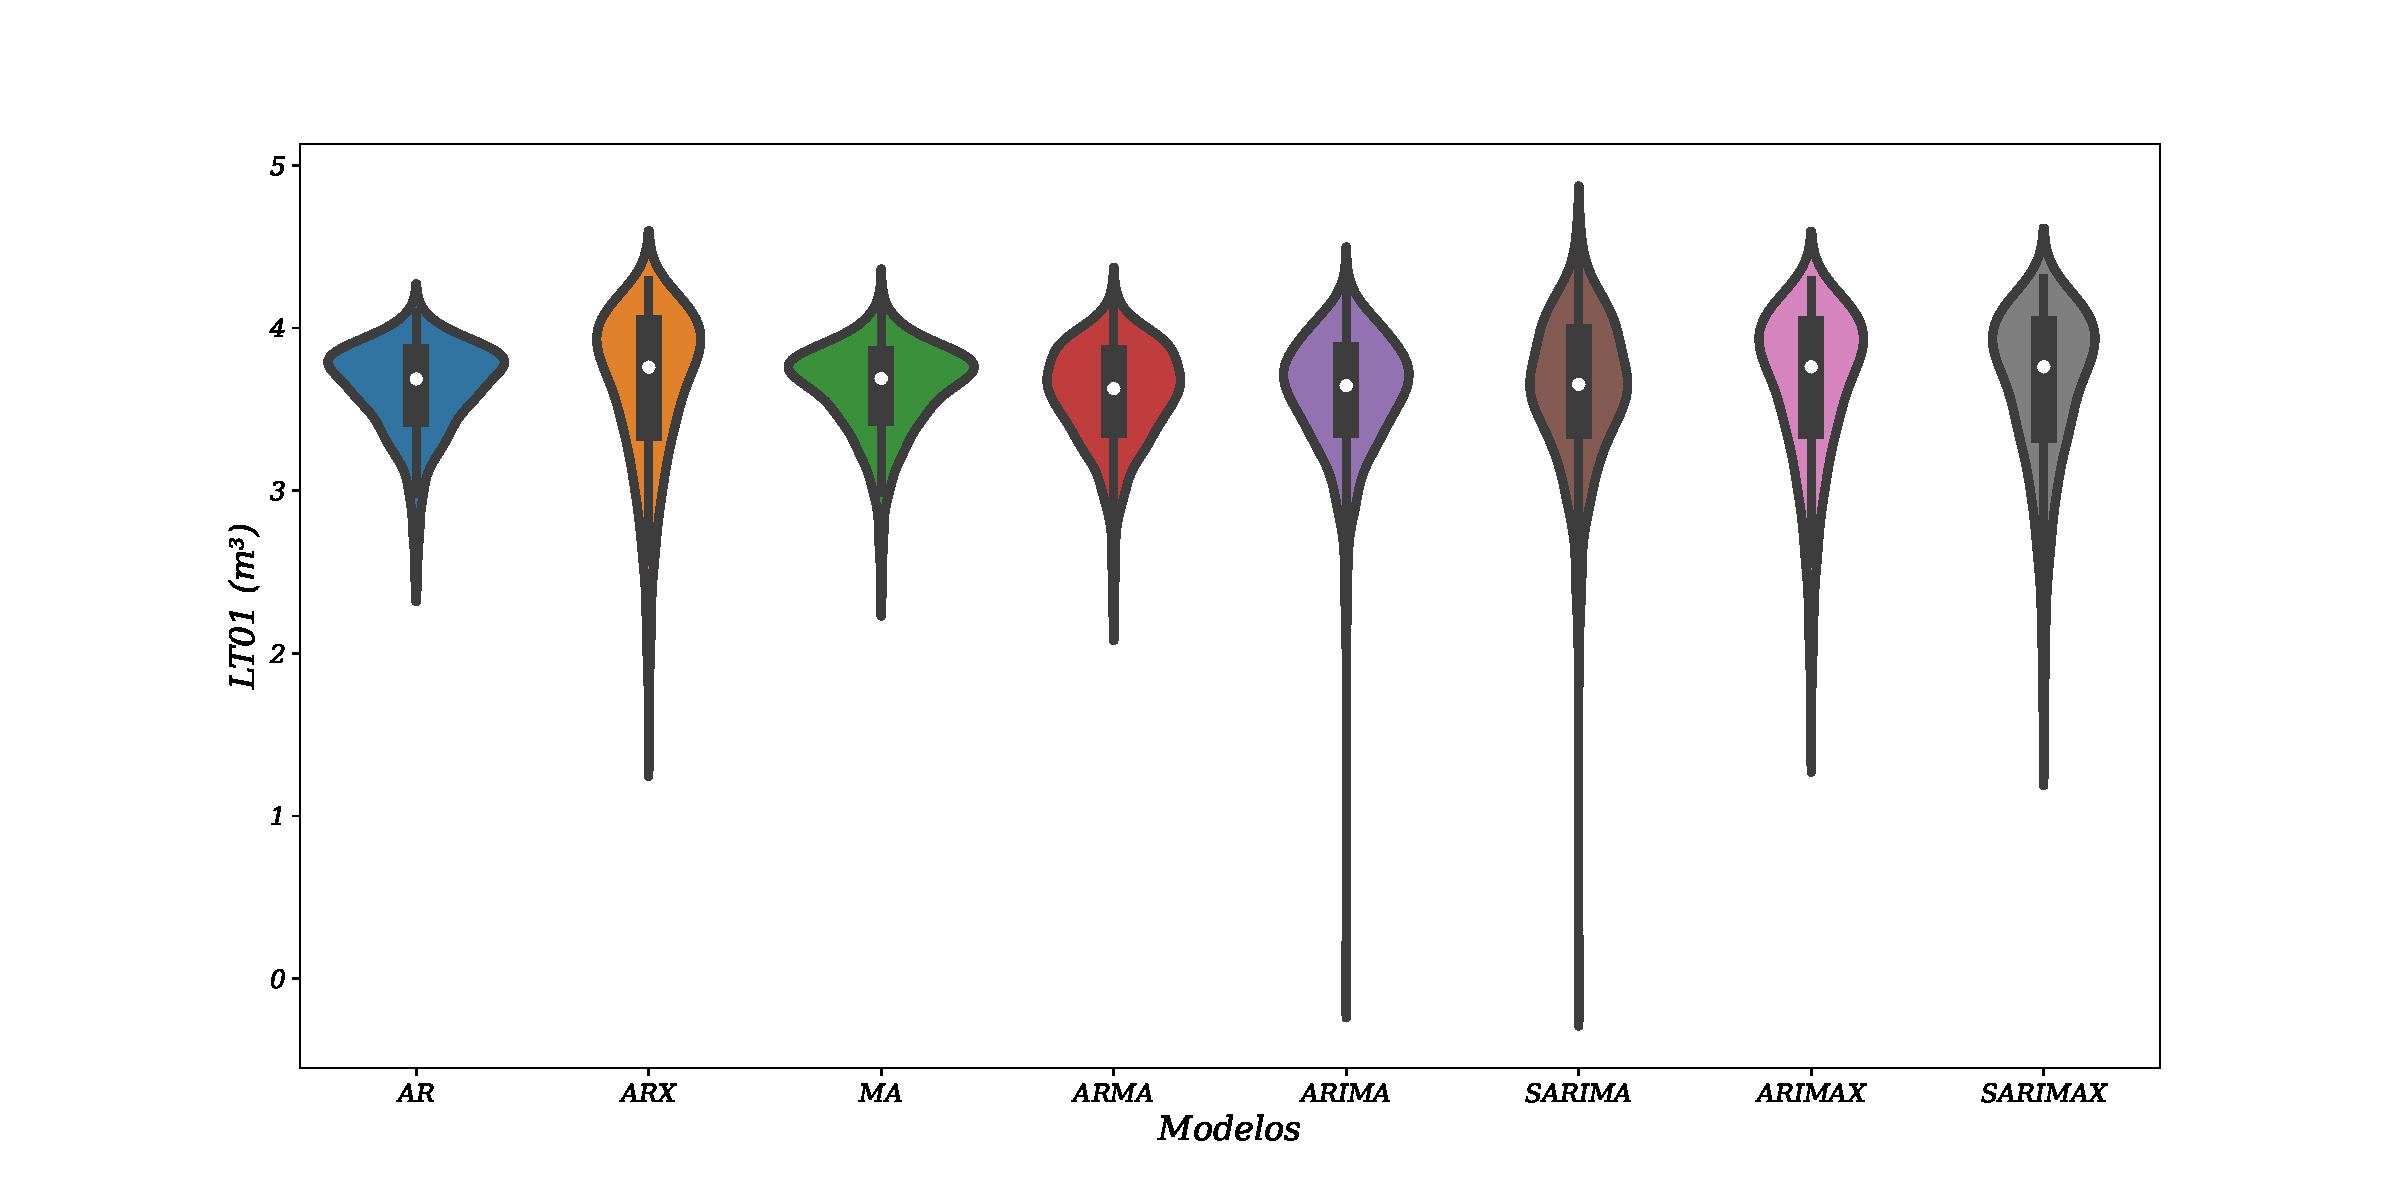
\includegraphics[width=\linewidth]{Resultados/Figuras/modelos-arima}
	
	
\end{figure}

Na Figura \ref{fig:violin-lr-xgb-lgbm-rf}, é feita uma comparação entre os modelos de gradiente e regressor. Esses modelos, por serem mais robustos e utilizar técnicas de otimização mais avançadas, mostram-se superiores aos modelos comparados. O modelo XGBoost, em particular, é identificado como superior em relação aos outros modelos na análise.

\begin{figure}[!htb]
	\centering
	\caption{Comparação de modelos de regressão}\label{fig:violin-lr-xgb-lgbm-rf}
	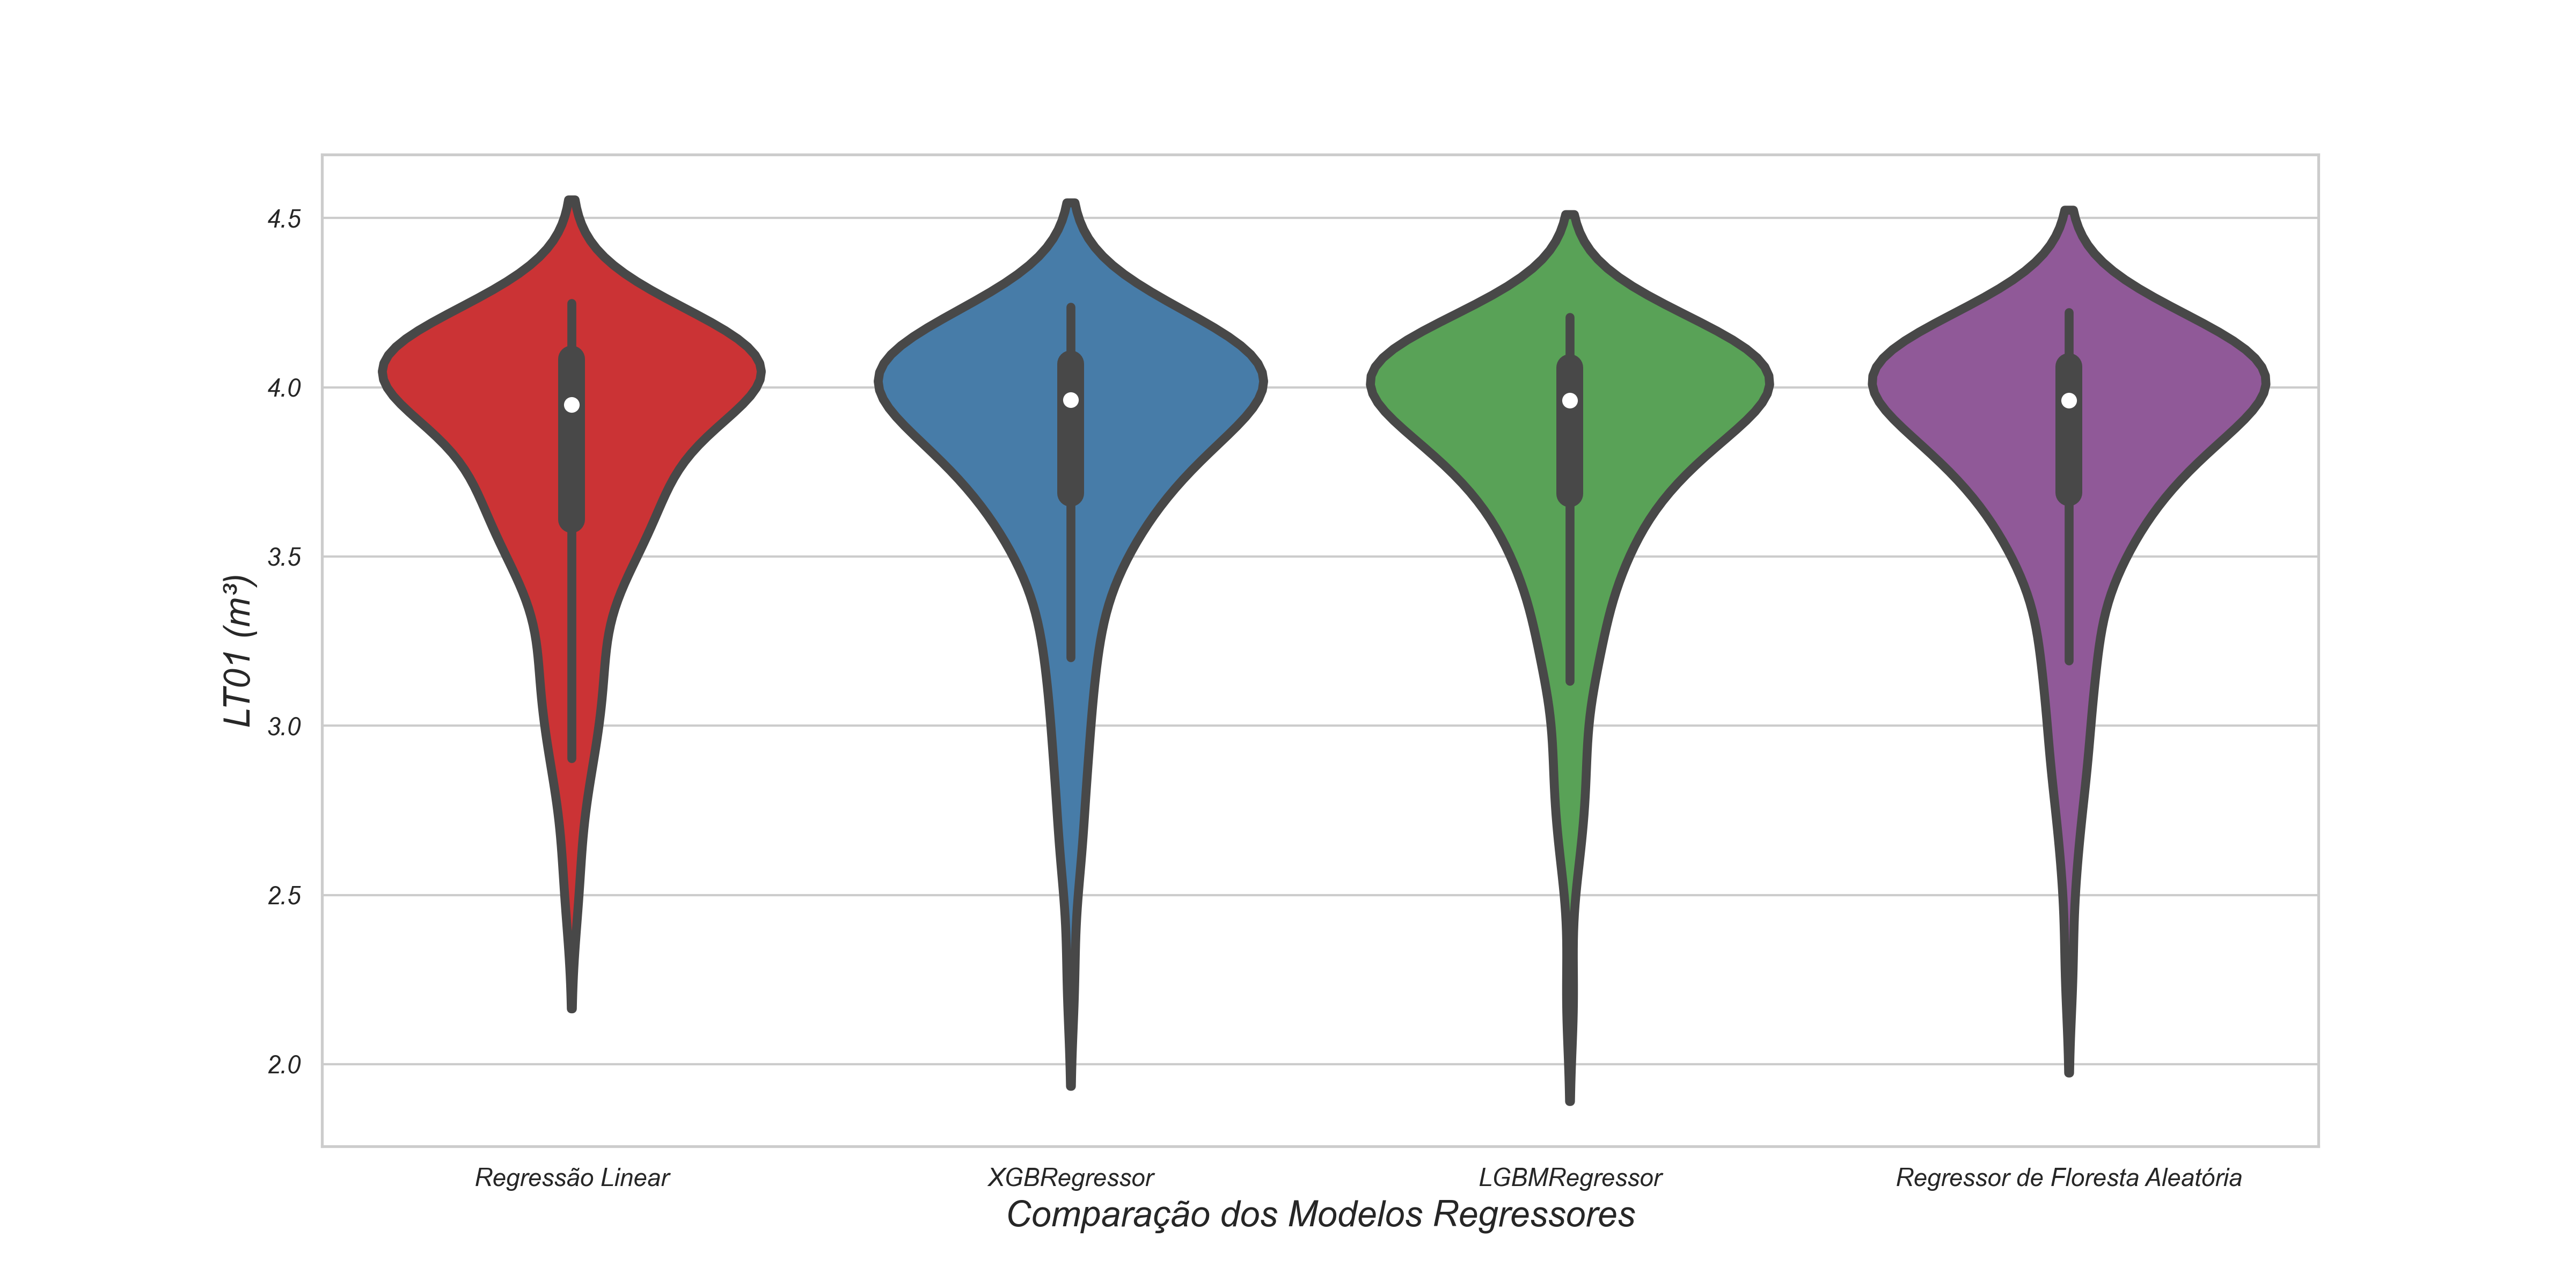
\includegraphics[width=\linewidth]{Resultados/Figuras/violin-LR-XGB-LGBM-RF}
	
\end{figure}

Na Figura \ref{fig:rrmse_comparar}, nota-se que todos os modelos trabalhados aqui, exceto o modelo LR, foram comparados em relação às métricas de desempenho. Mesmo sendo muito robustos, esses modelos não conseguiram obter um resultado tão bom quanto o RNN.
\begin{figure}[!htb]
	\centering
	\caption{Comparação dos modelos na métrica RRMSE\label{fig:rrmse_comparar}}
	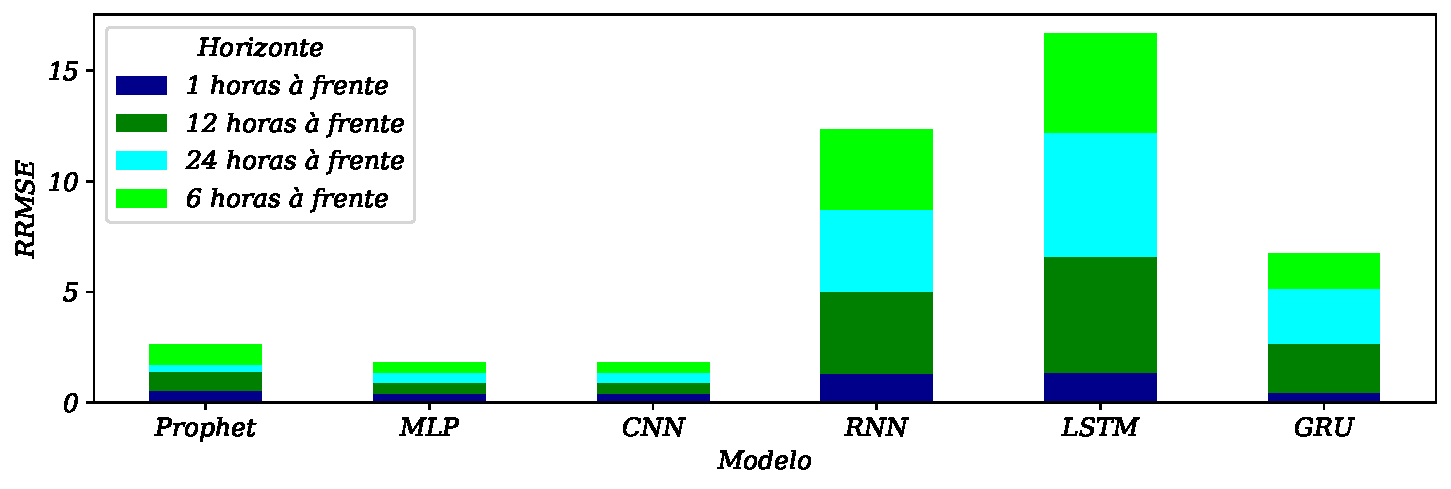
\includegraphics[width=\linewidth]{Resultados/Figuras/rrmse_comparar}
\end{figure}

\begin{figure}[!htb]
	\centering
	\caption{Comparação dos modelos nas métricas sMAPE, MAE e RRMSE\label{fig:basic_comparar}}
	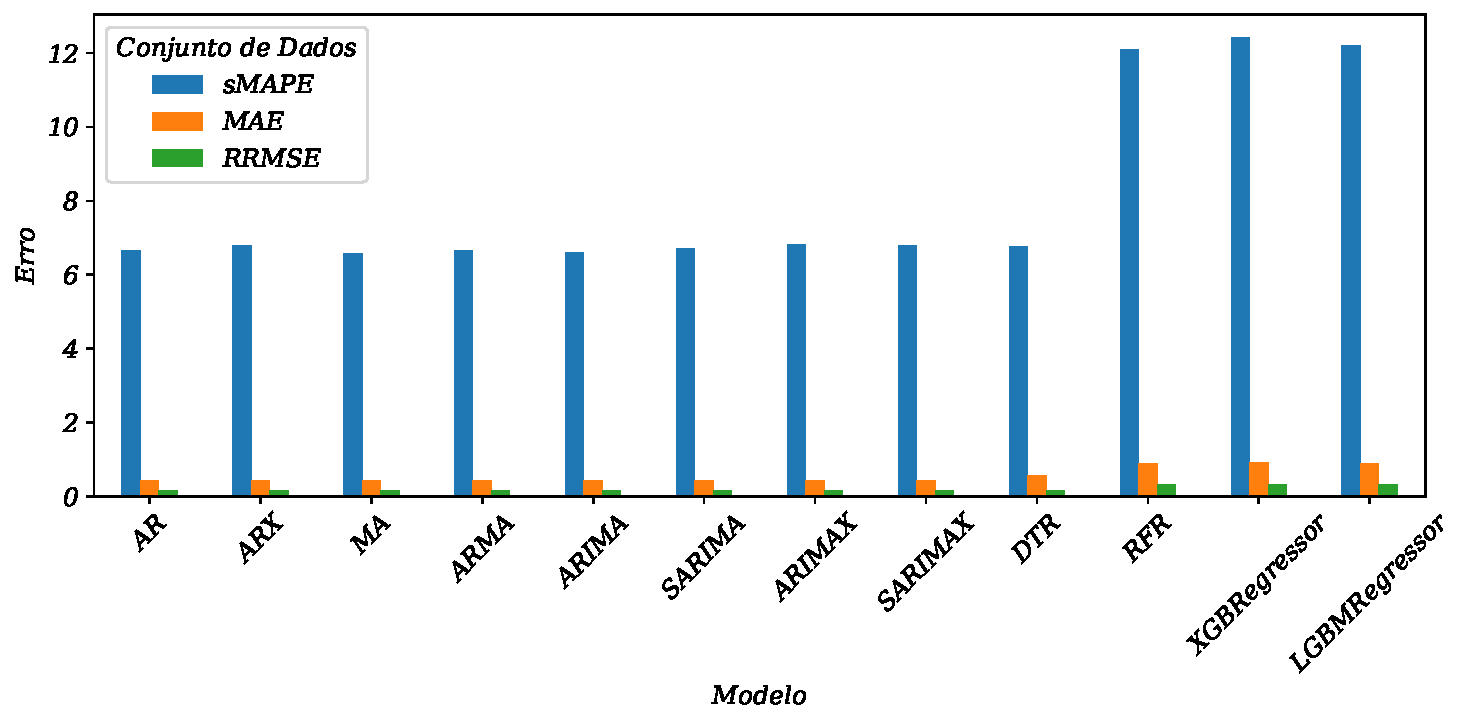
\includegraphics[width=\linewidth]{Resultados/Figuras/basic_comparar}
\end{figure}



A avaliação da eficácia dos modelos ARIMA em previsões de longo prazo emprega o teste de Ljung-Box, conforme detalhado nas Tabelas \ref{tb:lbtrn} a \ref{tb:lbcm} ilustram a acurácia dos modelos ARIMA ao longo do tempo, com valores menores sendo destacados em \textbf{negrito}  para facilitar a interpretação. Modelos como ARX, ARIMAX e SARIMAX, que incorporam variáveis exógenas, demonstram um desempenho superior nesse contexto. Esses modelos não lineares apresentam uma capacidade de previsão robusta em horizontes temporais mais longos, diferenciando-se positivamente dos outros modelos ARIMA. Na Figura \ref{fig:modelos-arima}, são selecionados os modelos ARIMA e seus antecessores. Esses modelos têm suas limitações, tanto para horizontes de previsão de curto prazo quanto para horizontes de longo prazo. Nessa comparação no gráfico de violino, são combinados vários outros gráficos em um só, como o gráfico de barras e o \textit{boxplot}. Esse gráfico pode fornecer várias informações, mas o objetivo aqui é identificar apenas o melhor modelo entre os modelos ARIMA.

Como essa série não apresentou uma estacionariedade bem definida e os dados não a tornaram estacionária, os modelos que não têm sazonalidade mostraram-se superiores, tais como AR, MA, ARX, ARMA, ARIMA e ARIMAX. O modelo ARIMAX demonstrou ser bastante robusto para este caso, mas mesmo assim, modelos mais básicos como AR e MA ainda apresentaram resultados melhores.

\begin{table}[H]
	\centering		
	\caption{Comparação dos modelos Ljung Box: Modelos ARIMA com defasagem de 10 para previsão de longo prazo na demanda de água}
	
	\begin{subtable}{0.46\linewidth}
		\centering
		\caption{\textbf{Treinamento}} \label{tb:lbtrn}
		\begin{tabular}{@{}ccc@{}}
			\toprule
			\multirow{5}{*}{\begin{tabular}[c]{@{}c@{}}Ljung \\ Box\end{tabular}} & \multirow{5}{*}{\begin{tabular}[c]{@{}c@{}}Estatística\\ de Teste\end{tabular}} & \multirow{5}{*}{\begin{tabular}[c]{@{}c@{}}Valor \\ De p\end{tabular}} \\
			& & \\
			& & \\
			& & \\
			& & \\ \midrule
		ARX & 59,677 & \textbf{0,000} \\
		AR & 52,312 & \textbf{0,265} \\
		MA & 57,268 & \textbf{0,000} \\
		ARMA & \textbf{6,945} & \textbf{0,731} \\
		ARIMA & 16,724 & 0,081 \\
		SARIMA & 48,505 & \textbf{0,000} \\
		ARIMAX & 89,931 & \textbf{0,000} \\
		SARIMAX & 29,093 & \textbf{0,000} \\ \bottomrule
		\end{tabular}
	\end{subtable}
	\hfill
	\begin{subtable}{0.46\linewidth}
		\centering
		\caption{\textbf{Teste}} \label{tb:lbtst}
		\begin{tabular}{@{}ccc@{}}
			\toprule
			\multirow{5}{*}{\begin{tabular}[c]{@{}c@{}}Ljung \\ Box\end{tabular}} & \multirow{5}{*}{\begin{tabular}[c]{@{}c@{}}Estatística\\ de Teste\end{tabular}} & \multirow{5}{*}{\begin{tabular}[c]{@{}c@{}}Valor \\ De p\end{tabular}} \\
			& & \\
			& & \\
			& & \\
			& & \\ \midrule
			ARX & 47,177 & \textbf{0,000} \\
			AR & 49,965 & 0,444 \\
			MA & 77,884 & \textbf{0,000} \\
			ARMA & \textbf{1,545} & 0,999 \\
			ARIMA & \textbf{5,354} & 0,866 \\
			SARIMA & 24,663 & \textbf{0,006} \\
			ARIMAX & 36,738 & \textbf{0,000} \\
			SARIMAX & 21,236 & \textbf{0,020} \\ \bottomrule
		\end{tabular}
	\end{subtable}
	
	\vspace{1em}
	
	\begin{subtable}{0.46\linewidth}
		\centering
		\caption{\textbf{Validação}} \label{tb:lbvld}
		\begin{tabular}{@{}ccc@{}}
			\toprule
			\multirow{5}{*}{\begin{tabular}[c]{@{}c@{}}Ljung \\ Box\end{tabular}} & \multirow{5}{*}{\begin{tabular}[c]{@{}c@{}}Estatística\\ de Teste\end{tabular}} & \multirow{5}{*}{\begin{tabular}[c]{@{}c@{}}Valor \\ De p\end{tabular}} \\
			& & \\
			& & \\
			& & \\
			& & \\ \midrule
			ARX & \textbf{5,108} & 0,884 \\
			AR & 4,360 & 0,930 \\
			MA & 46,252 & \textbf{0,000} \\
			ARMA & \textbf{7,515} & 0,676 \\
			ARIMA & \textbf{7,738} & 0,654 \\
			SARIMA & 28,998 & \textbf{0,001} \\
			ARIMAX & \textbf{6,115} & \textbf{0,000} \\
			SARIMAX & \textbf{4,443} & 0,925 \\ \bottomrule
		\end{tabular}
	\end{subtable}
	\hfill
	\begin{subtable}{0.46\linewidth}
		\centering
		\caption{\textbf{Inteiro}} \label{tb:lbcm}
		\begin{tabular}{@{}ccc@{}}
			\toprule
			\multirow{5}{*}{\begin{tabular}[c]{@{}c@{}}Ljung \\ Box\end{tabular}} & \multirow{5}{*}{\begin{tabular}[c]{@{}c@{}}Estatística\\ de Teste\end{tabular}} & \multirow{5}{*}{\begin{tabular}[c]{@{}c@{}}Valor \\ De p\end{tabular}} \\
			& & \\
			& & \\
			& & \\
			& & \\ \midrule
		ARX & 48,870 & \textbf{0,000} \\
		AR & 49,432 & \textbf{0,035} \\
		MA & 57,629 & \textbf{0,000} \\
		ARMA & \textbf{10,053} & \textbf{0,436} \\
		ARIMA & \textbf{10,053} & \textbf{0,436} \\
		SARIMA & \textbf{10,053} & \textbf{0,436} \\
		ARIMAX & 70,458 & \textbf{0,000} \\
		SARIMAX & \textbf{2,897} & \textbf{0,000} \\ \bottomrule
		\end{tabular}
	\end{subtable}
	
	
	\vspace{0.5cm}
	
\end{table}





